\documentclass[otchet]{SCWorks}
% Тип обучения (одно из значений):
%    bachelor   - бакалавриат (по умолчанию)
%    spec       - специальность
%    master     - магистратура
% Форма обучения (одно из значений):
%    och        - очное (по умолчанию)
%    zaoch      - заочное
% Тип работы (одно из значений):
%    coursework - курсовая работа (по умолчанию)
%    referat    - реферат
%  * otchet     - универсальный отчет
%  * nirjournal - журнал НИР
%  * digital    - итоговая работа для цифровой кафедры
%    diploma    - дипломная работа
%    pract      - отчет о научно-исследовательской работе
%    autoref    - автореферат выпускной работы
%    assignment - задание на выпускную квалификационную работу
%    review     - отзыв руководителя
%    critique   - рецензия на выпускную работу

% * Добавлены вручную. За вопросами к @mchernigin
\usepackage{preamble}
\floatplacement{figure}{H}
\setkeys{Gin}{width=1.2\textwidth}
\setminted{breaklines=true, breakanywhere=true}

\begin{document}

% Кафедра (в родительном падеже)
\chair{математической кибернетики и компьютерных наук}

% Тема работы
\title{Разработка схемы индексирования данных в базе}

% Курс
\course{3}

% Группа
\group{351}

% Факультет (в родительном падеже) (по умолчанию "факультета КНиИТ")
\department{факультета компьютерных наук и информационных технологий}

% Специальность/направление код - наименование
% \napravlenie{02.03.02 "--- Фундаментальная информатика и информационные технологии}
% \napravlenie{02.03.01 "--- Математическое обеспечение и администрирование информационных систем}
% \napravlenie{09.03.01 "--- Информатика и вычислительная техника}
\napravlenie{09.03.04 "--- Программная инженерия}
% \napravlenie{10.05.01 "--- Компьютерная безопасность}

% Для студентки. Для работы студента следующая команда не нужна.
\studenttitle{студентки}

% Фамилия, имя, отчество в родительном падеже
\author{Потапкиной Маргариты Андреевны}

% Заведующий кафедрой 
\chtitle{доцент, к.\,ф.-м.\,н.}
\chname{С.\,В.\,Миронов}

% Руководитель ДПП ПП для цифровой кафедры (перекрывает заведующего кафедры)
% \chpretitle{
%     заведующий кафедрой математических основ информатики и олимпиадного\\
%     программирования на базе МАОУ <<Ф"=Т лицей №1>>
% }
% \chtitle{г. Саратов, к.\,ф.-м.\,н., доцент}
% \chname{Кондратова\, Ю.\,Н.}

% Научный руководитель (для реферата преподаватель проверяющий работу)
\satitle{доцент, к.\,ф.-м.\,н.}
\saname{И.\,А.\,Батраева}

% Руководитель практики от организации (руководитель для цифровой кафедры)
\patitle{доцент, к.\,ф.-м.\,н.}
\paname{И.\,А.\,Батраева}

% Руководитель НИР
\nirtitle{доцент, к.\,п.\,н.} % степень, звание
\nirname{И.\,А.\,Батраева}

% Семестр (только для практики, для остальных типов работ не используется)
\term{5}

% Наименование практики (только для практики, для остальных типов работ не
% используется)
\practtype{учебная}

% Продолжительность практики (количество недель) (только для практики, для
% остальных типов работ не используется)
\duration{2}

% Даты начала и окончания практики (только для практики, для остальных типов
% работ не используется)
\practStart{01.07.2024}
\practFinish{13.01.2024}

% Год выполнения отчета
\date{2026}

\maketitle

% Включение нумерации рисунков, формул и таблиц по разделам (по умолчанию -
% нумерация сквозная) (допускается оба вида нумерации)
\secNumbering

\tableofcontents

% Раздел "Обозначения и сокращения". Может отсутствовать в работе
% \abbreviations
% \begin{description}
%     \item ... "--- ...
%     \item ... "--- ...
% \end{description}

% Раздел "Определения". Может отсутствовать в работе
% \definitions

% Раздел "Определения, обозначения и сокращения". Может отсутствовать в работе.
% Если присутствует, то заменяет собой разделы "Обозначения и сокращения" и
% "Определения"
% \defabbr

\intro
В ходе выполнения работы была разработана, реализована и протестирована схема индексирования данных в базе.

Были изучены следующие типы индексов:
\begin{enumerate}
    \item Простой (без каких-либо модификаторов/предложений);
    \item Уникальный;
    \item Составной;
    \item Индексы с использованием выражений,
    \item Покрывающий;
    \item Частичный;
    \item Частичный покрывающий.
\end{enumerate}

Для тех индексов, где это технически возможно, были реализованы оба варианта индекса: через B"=Tree и Hash. В противном случае использовался только B"=Tree;

Также были реализованы следующие типы запросов:
\begin{enumerate}
\item Запросы c использованием различных видов соединений таблиц;
\item Фильтрация данных в запросах с использованием предикатов: EXISTS, IN, ALL, SOME/ANY, BETWEEN, LIKE, ILIKE;
\item Запросы с использованием функций для работы со строками: REPLACE, SUBSTRING, OVERLAY;
\item Запросы с использованием функций даты и времени DATE\_PART, арифметические операции с датами, CURRENT\_TIMESTAMP с уточнением временной зоны и без;
\item Запросы с использованием агрегатных функций, группировок GROUP BY и фильтрации групп HAVING
\item Вложенные запросы;
\item Запросы с использованием UNION и INTERSECT.
\end{enumerate}

Для различных типов запросов была сначала измерена скорость их работы без использования индексов. Затем был разработан соответствующий индекс, после чего был вновь проведён замер скорости работы. В результате индексы позволили в значительной степени оптимизировать запросы.


\section{Простой индекс (без каких"=либо модификаторов/предложений)}

\subsection{B"=Tree}

\subsubsection{Запрос 1}

\begin{enumerate}
\item Код запроса:
\begin{minted}{sql}
EXPLAIN ANALYZE
SELECT students.name, students.surname, grades.mark
FROM students
LEFT JOIN grades ON grades.student_id = students.id 
WHERE students.surname = 'Иванов_778';
\end{minted}
\item Какие типы запросов реализует?
\begin{itemize}
    \item запросы с использованием различных видов соединений таблиц (LEFT JOIN).
\end{itemize}
\item Скриншот планов выполнения запросов без индекса:
\begin{figure}
\centering
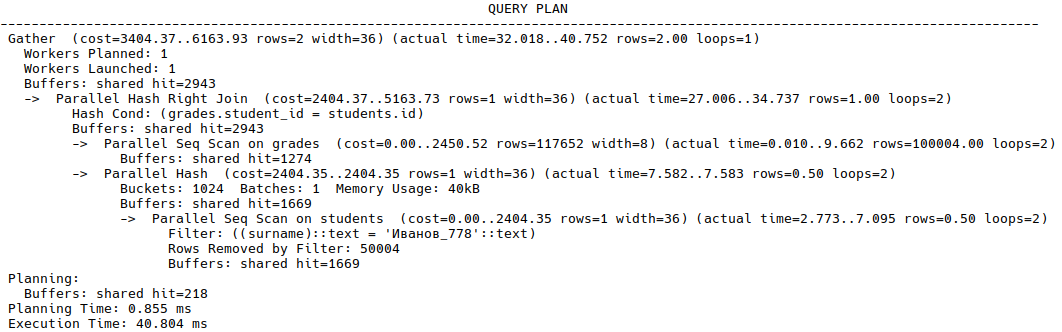
\includegraphics{q1p1.png}
\end{figure}
\item SQL"=код спроектированных индексов:
\begin{minted}{sql}
CREATE INDEX idx_surname ON students(surname);
CREATE INDEX idx_student_id ON grades(student_id);
\end{minted}
\item Скриншот планов выполнения запросов с индексом:
\begin{figure}
\centering
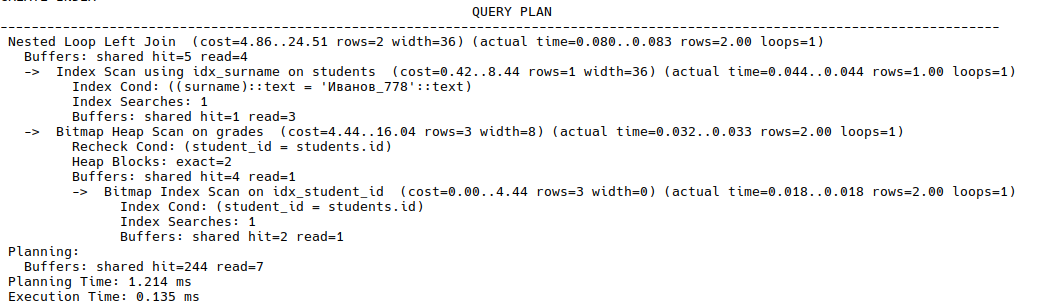
\includegraphics{q1p2.png}
\end{figure}
\end{enumerate}

\subsubsection{Запрос 2}

\begin{enumerate}
\item Код запроса:
\begin{minted}{sql}
EXPLAIN ANALYZE
SELECT name, surname, birth_date
FROM students
WHERE birth_date = (SELECT MIN (birth_date) FROM students);
\end{minted}
\item Какие типы запросов реализует?
\begin{itemize}
    \item вложенные запросы;
    \item запросы с использованием агрегатных функций.
\end{itemize}
\item Скриншот планов выполнения запросов без индекса:
\begin{figure}
\centering
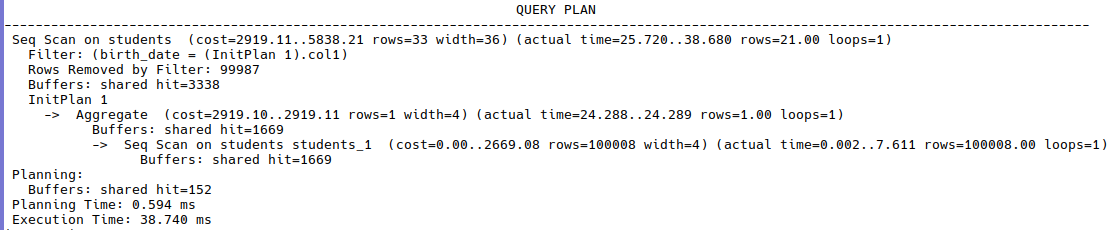
\includegraphics{q4p1.png}
\end{figure}
\item SQL"=код спроектированных индексов:
\begin{minted}{sql}
CREATE INDEX idx_birth_date ON students(birth_date);
\end{minted}
\item Скриншот планов выполнения запросов с индексом:
\begin{figure}
\centering
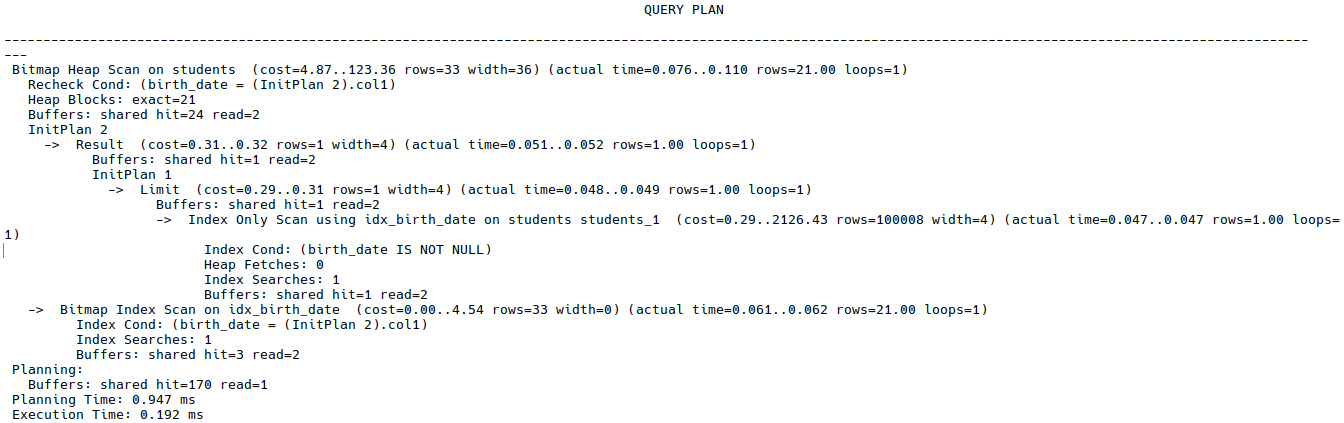
\includegraphics{q4p2.png}
\end{figure}
\end{enumerate}

\subsubsection{Запрос 3}

\begin{enumerate}
\item Код запроса:
\begin{minted}{sql}
EXPLAIN ANALYZE
SELECT groups.group_number, s1.students_count
FROM ( SELECT group_id, COUNT(*) AS students_count
       FROM students
       GROUP BY group_id
       HAVING COUNT(*) > 1 ) s1
INNER JOIN groups ON groups.id = s1.group_id;
\end{minted}
\item Какие типы запросов реализует?
\begin{itemize}
    \item запросы c использованием различных видов соединений таблиц;
    \item запросы с использованием агрегатных функций, группировок GROUP BY и фильтрации групп HAVING;
    \item вложенные запросы.
\end{itemize}
\item Скриншот планов выполнения запросов без индекса:
\begin{figure}
\centering
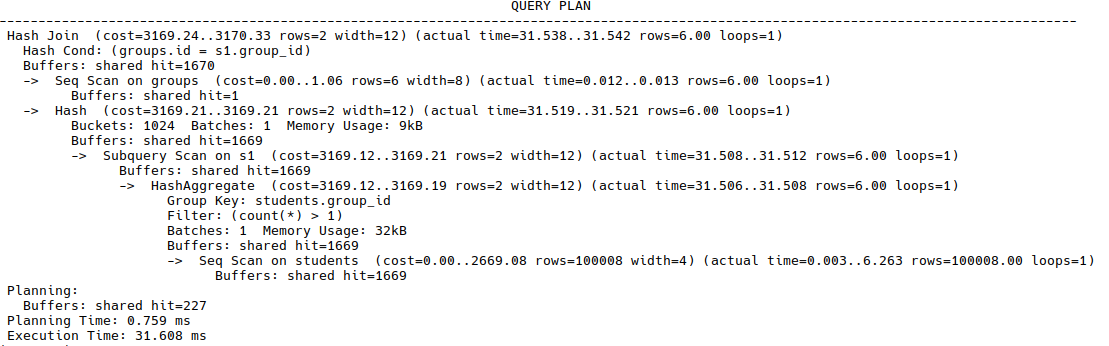
\includegraphics{q15p1.png}
\end{figure}
\item SQL"=код спроектированных индексов:
\begin{minted}{sql}
CREATE INDEX idx_group_id ON students(group_id);
\end{minted}
\item Скриншот планов выполнения запросов с индексом:
\begin{figure}
\centering
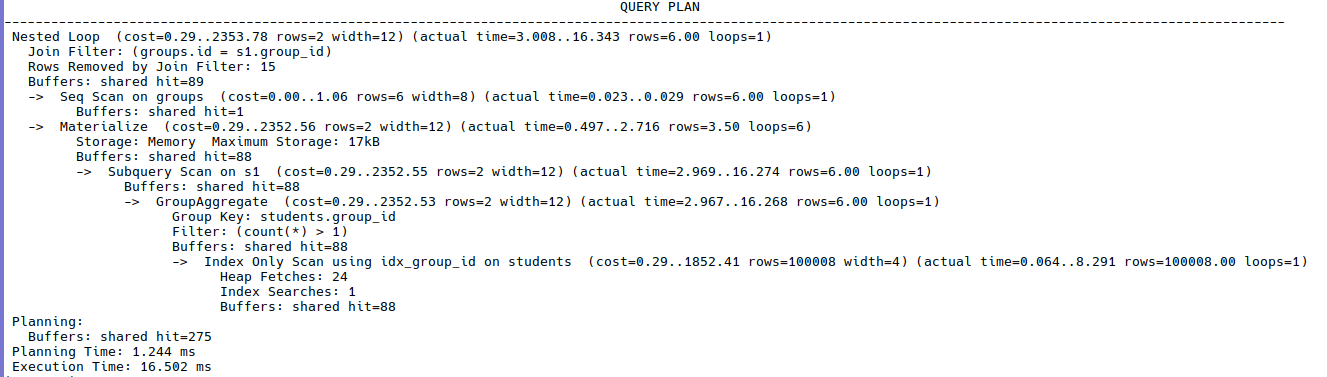
\includegraphics{q15p2.png}
\end{figure}
\end{enumerate}
\subsection{Hash}

\subsubsection{Запрос 1}

\begin{enumerate}
\item Код запроса:
\begin{minted}{sql}
EXPLAIN ANALYZE
SELECT s1.surname, s2.surname, s1.birth_date
FROM students s1
INNER JOIN students s2 ON s1.birth_date = s2.birth_date AND s1.id < s2.id
WHERE s1.birth_date = '2004-05-12';
\end{minted}
\item Какие типы запросов реализует?
\begin{itemize}
\item запросы с использованием различных видов соединений таблиц (INNER JOIN).
\end{itemize}
\item Скриншот планов выполнения запросов без индекса:
\begin{figure}
\centering
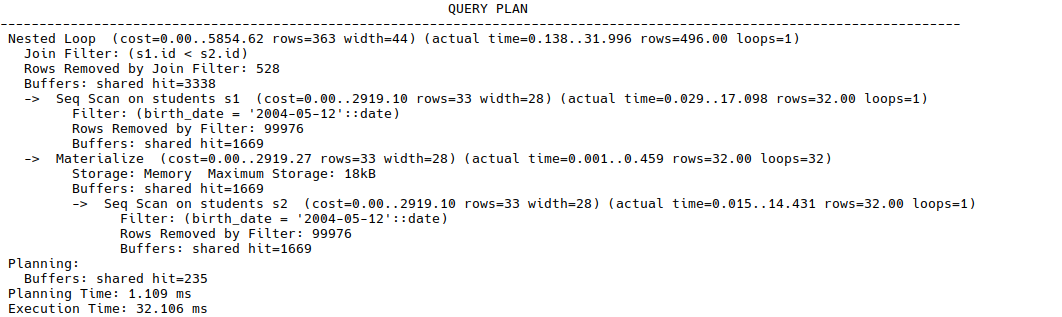
\includegraphics{q2p1.png}
\end{figure}
\item SQL"=код спроектированных индексов:
\begin{minted}{sql}
CREATE INDEX idx_birth_date ON students USING HASH(birth_date);
\end{minted}
\item Скриншот планов выполнения запросов с индексом:
\begin{figure}
\centering
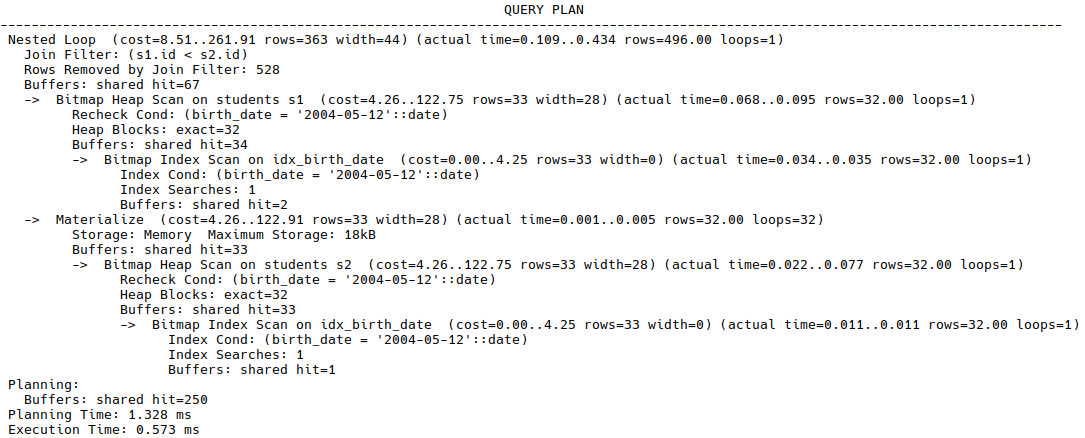
\includegraphics{q2p2.png}
\end{figure}
\end{enumerate}


\section{Уникальный индекс}
\subsection{B"=Tree}

\subsubsection{Запрос 1}

\begin{enumerate}
\item Код запроса:
\begin{minted}{sql}
EXPLAIN ANALYZE
SELECT name, surname, patronymic
FROM teachers
WHERE surname IN ('Колдунов', 'Сахно', 'Миронов');
\end{minted}
\item Какие типы запросов реализует?
\begin{itemize}
    \item фильтрация данных в запросах с использованием предикатов: IN.
\end{itemize}
\item Скриншот планов выполнения запросов без индекса:
\begin{figure}
\centering
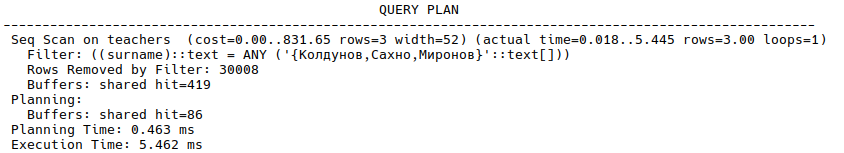
\includegraphics{q5p1.png}
\end{figure}
\item SQL"=код спроектированных индексов:
\begin{minted}{sql}
CREATE UNIQUE INDEX idx_teachers_surname ON teachers(surname);
\end{minted}
\item Скриншот планов выполнения запросов с индексом:
\begin{figure}
\centering
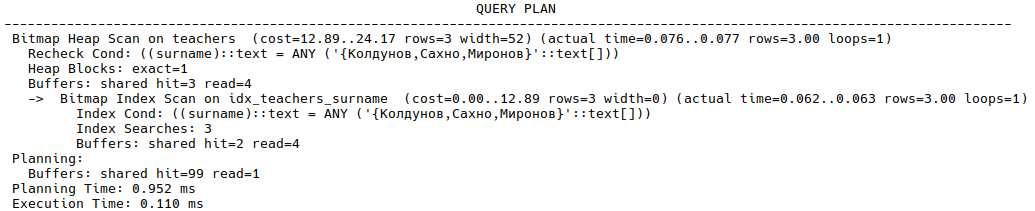
\includegraphics{q5p2.png}
\end{figure}
\end{enumerate}


\section{Составной индекс}
\subsection{B"=Tree}

\subsubsection{Запрос 1}

\begin{enumerate}
\item Код запроса:
\begin{minted}{sql}
EXPLAIN ANALYZE
SELECT surname, name FROM students
WHERE group_id = ANY (SELECT id FROM groups WHERE course_number = 3) AND name = 'Иван' AND surname LIKE 'Иванов%';
\end{minted}
\item Какие типы запросов реализует?
\begin{itemize}
    \item фильтрация данных в запросах с использованием предикатов: ANY, LIKE;
    \item вложенные запросы.
\end{itemize}
\item Скриншот планов выполнения запросов без индекса:
\begin{figure}
\centering
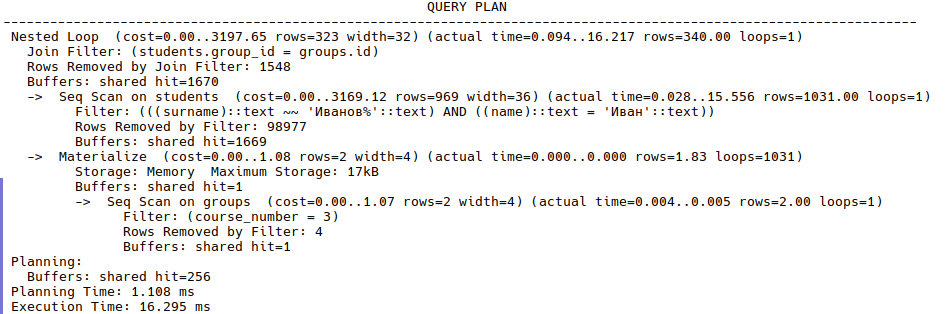
\includegraphics{q12p1.png}
\end{figure}
\item SQL"=код спроектированных индексов:
\begin{minted}{sql}
CREATE INDEX idx_surname_group_id ON students(group_id, name, surname varchar_pattern_ops);
\end{minted}
\item Скриншот планов выполнения запросов с индексом:
\begin{figure}
\centering
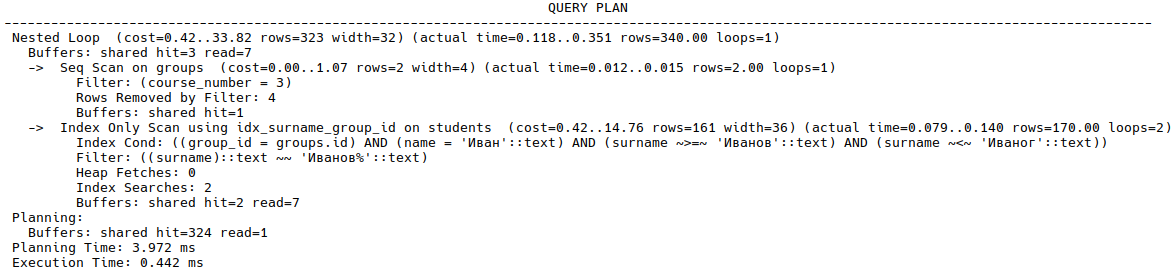
\includegraphics{q12p2.png}
\end{figure}
\end{enumerate}


\section{Индексы с использованием выражений}
\subsection{B"=Tree}

\subsubsection{Запрос 1}

\begin{enumerate}
\item Код запроса:
\begin{minted}{sql}
EXPLAIN ANALYZE
SELECT REPLACE(CAST(birth_date as VARCHAR), '-', '.') as str_date FROM students
WHERE DATE_PART('year', birth_date) = 2000;
\end{minted}
\item Какие типы запросов реализует?
\begin{itemize}
    \item запросы с использованием функций для работы со строками: REPLACE;
    \item запросы с использованием функций даты и времени: DATE\_PART.
\end{itemize}
\item Скриншот планов выполнения запросов без индекса:
\begin{figure}
\centering
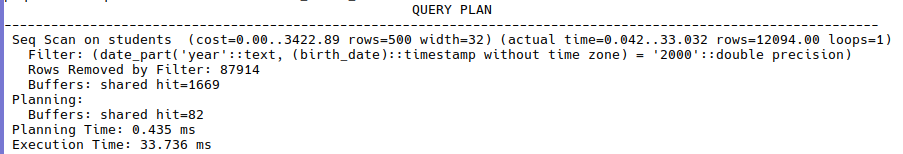
\includegraphics{q8p1.png}
\end{figure}
\item SQL"=код спроектированных индексов:
\begin{minted}{sql}
CREATE INDEX idx_birth_year ON students(DATE_PART('year', birth_date));
\end{minted}
\item Скриншот планов выполнения запросов с индексом:
\begin{figure}
\centering
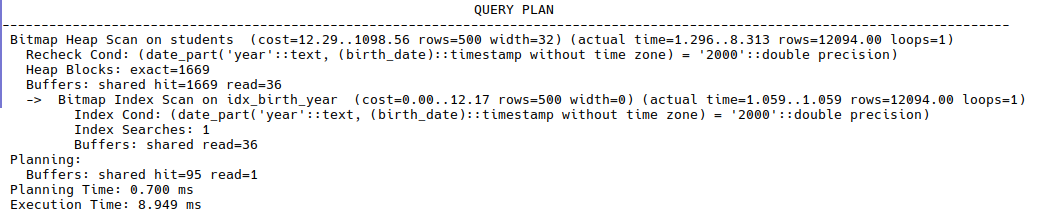
\includegraphics{q8p2.png}
\end{figure}
\end{enumerate}

\subsubsection{Запрос 2 (также относится к покрывающему индексу)}

\begin{enumerate}
\item Код запроса:
\begin{minted}{sql}
EXPLAIN ANALYZE
SELECT surname, name, birth_date
FROM students
WHERE DATE_PART('month', birth_date) = EXTRACT (MONTH FROM CURRENT_DATE + INTERVAL '1 month');
\end{minted}
\item Какие типы запросов реализует?
\begin{itemize}
    \item запросы с использованием функций даты и времени DATE\_PART, арифметические операции с датами.
\end{itemize}
\item Скриншот планов выполнения запросов без индекса:
\begin{figure}
\centering
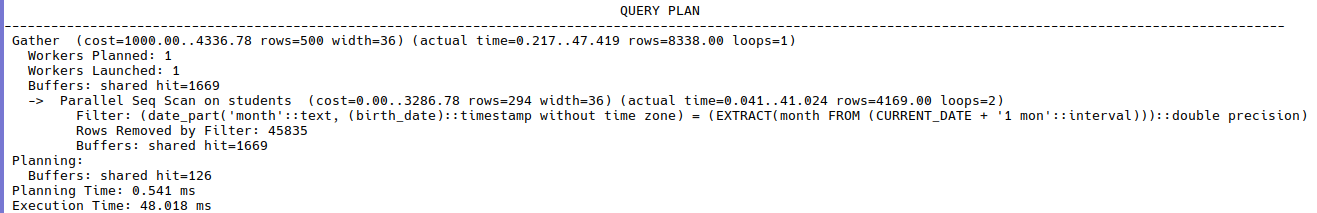
\includegraphics{q13p1.png}
\end{figure}
\item SQL"=код спроектированных индексов:
\begin{minted}{sql}
CREATE INDEX idx_birth_month ON students(DATE_PART('month', birth_date)) INCLUDE (surname, name);
\end{minted}
\item Скриншот планов выполнения запросов с индексом:
\begin{figure}
\centering
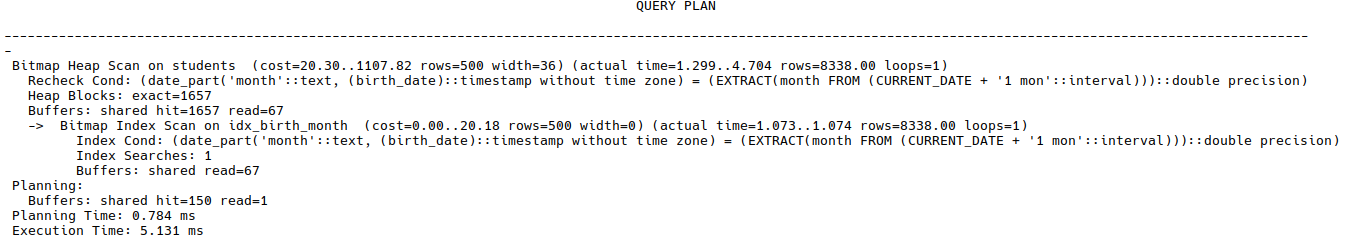
\includegraphics{q13p2.png}
\end{figure}
\end{enumerate}

\subsection{Hash}

\subsubsection{Запрос 1}

\begin{enumerate}
\item Код запроса:
\begin{minted}{sql}
EXPLAIN ANALYZE
SELECT name, surname, snils FROM students
WHERE SUBSTRING(snils FROM 5 FOR 2) = '01';
\end{minted}
\item Какие типы запросов реализует?
\begin{itemize}
    \item запросы с использованием функций для работы со строками: SUBSTRING.
\end{itemize}
\item Скриншот планов выполнения запросов без индекса:
\begin{figure}
\centering
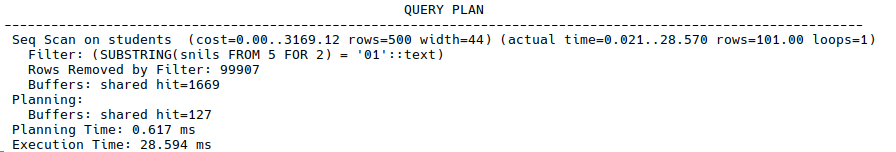
\includegraphics{q9p1.png}
\end{figure}
\item SQL"=код спроектированных индексов:
\begin{minted}{sql}
CREATE INDEX idx_snils ON students USING HASH(SUBSTRING(snils FROM 5 FOR 2));
\end{minted}
\item Скриншот планов выполнения запросов с индексом:
\begin{figure}
\centering
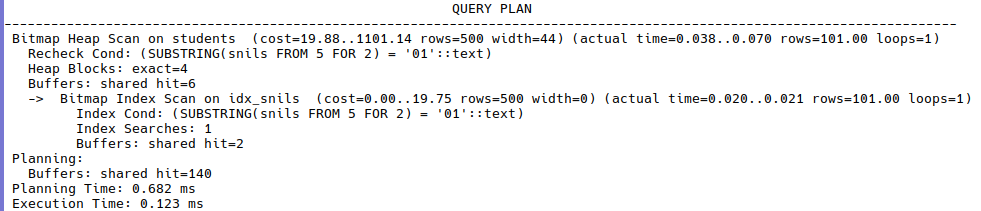
\includegraphics{q9p2.png}
\end{figure}
\end{enumerate}


\section{Покрывающий индекс}
\subsection{B"=Tree}

\subsubsection{Запрос 1}

\begin{enumerate}
\item Код запроса:
\begin{minted}{sql}
EXPLAIN ANALYZE
SELECT student_id FROM grades WHERE points = 94
UNION
SELECT student_id FROM student_orders WHERE order_date = '2025-10-26';
\end{minted}
\item Какие типы запросов реализует?
\begin{itemize}
    \item запросы с использованием UNION.
\end{itemize}
\item Скриншот планов выполнения запросов без индекса:
\begin{figure}
\centering
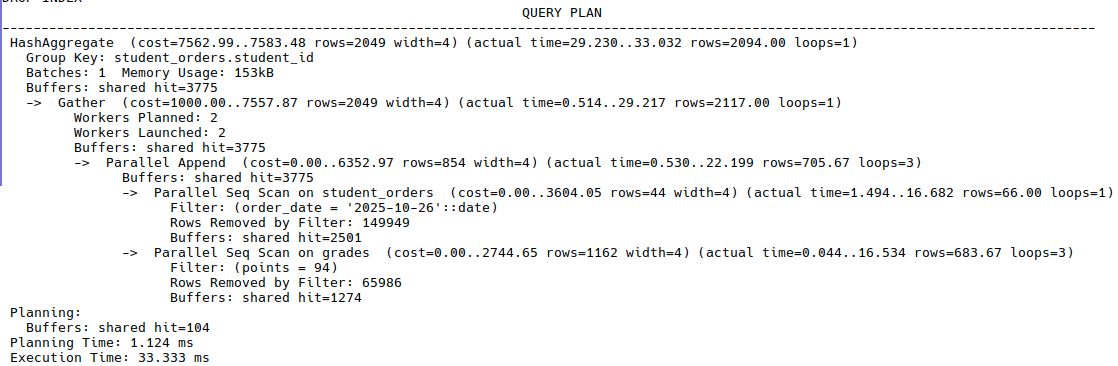
\includegraphics{q3p1.png}
\end{figure}
\item SQL"=код спроектированных индексов:
\begin{minted}{sql}
CREATE INDEX idx_points ON grades(points) INCLUDE (student_id);
CREATE INDEX idx_orders ON student_orders(order_date) INCLUDE (student_id);
\end{minted}
\item Скриншот планов выполнения запросов с индексом:
\begin{figure}
\centering
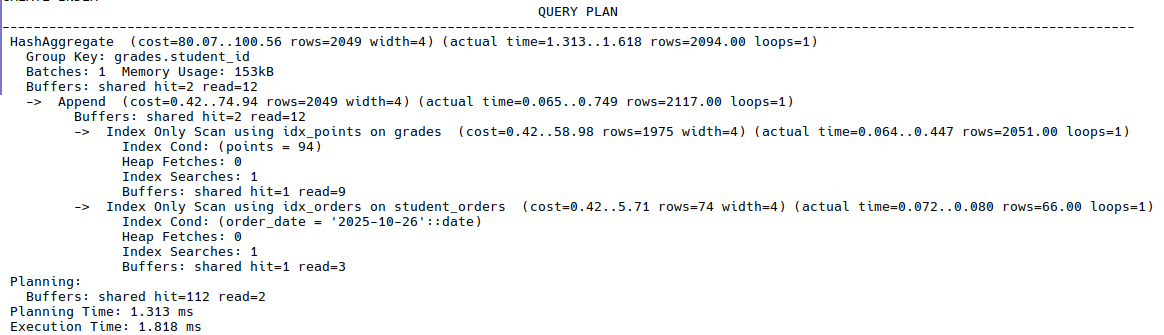
\includegraphics{q3p2.png}
\end{figure}
\end{enumerate}

\subsubsection{Запрос 2}

\begin{enumerate}
\item Код запроса:
\begin{minted}{sql}
EXPLAIN ANALYZE
SELECT name, surname, OVERLAY (passport PLACING '******' FROM 5 FOR 6) as hidden_passport FROM students
WHERE passport LIKE '63%';
\end{minted}
\item Какие типы запросов реализует?
\begin{itemize}
    \item фильтрация данных в запросах с использованием предикатов: LIKE;
    \item запросы с использованием функций для работы со строками: OVERLAY.
\end{itemize}
\item Скриншот планов выполнения запросов без индекса:
\begin{figure}
\centering
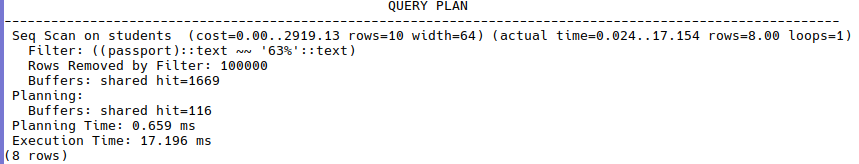
\includegraphics{q6p1.png}
\end{figure}
\item SQL"=код спроектированных индексов:
\begin{minted}{sql}
CREATE INDEX idx_passport ON students(passport varchar_pattern_ops) INCLUDE (name, surname);
\end{minted}
\item Скриншот планов выполнения запросов с индексом:
\begin{figure}
\centering
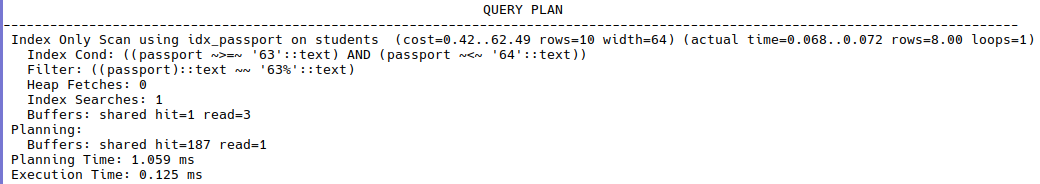
\includegraphics{q6p2.png}
\end{figure}
\end{enumerate}

\subsubsection{Запрос 3}

\begin{enumerate}
\item Код запроса:
\begin{minted}{sql}
EXPLAIN ANALYZE
SELECT subject_id, lecture_hours FROM study_plan_subject
WHERE study_plan_subject.subject_id = SOME (SELECT id FROM subjects WHERE name ILIKE '%мат%');
\end{minted}
\item Какие типы запросов реализует?
\begin{itemize}
    \item фильтрация данных в запросах с использованием предикатов: SOME, ILIKE;
    \item вложенные запросы.
\end{itemize}
\item Скриншот планов выполнения запросов без индекса:
\begin{figure}
\centering
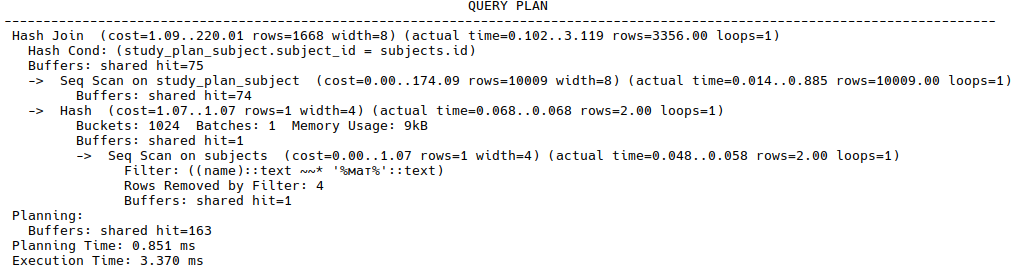
\includegraphics{q11p1.png}
\end{figure}
\item SQL"=код спроектированных индексов:
\begin{minted}{sql}
CREATE INDEX idx_subject_id ON study_plan_subject(subject_id) INCLUDE (lecture_hours);
\end{minted}
\item Скриншот планов выполнения запросов с индексом:
\begin{figure}
\centering
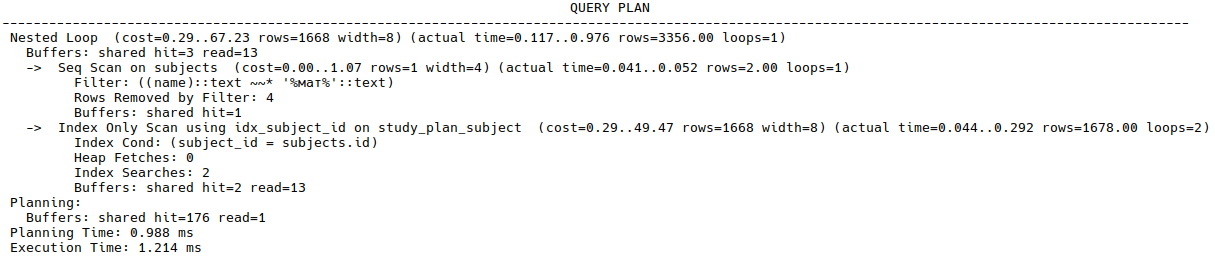
\includegraphics{q11p2.png}
\end{figure}
\end{enumerate}


\section{Частичный индекс}
\subsection{B"=Tree}

\subsubsection{Запрос 1}

\begin{enumerate}
\item Код запроса:
\begin{minted}{sql}
EXPLAIN ANALYZE
SELECT subject_id, lecture_hours FROM study_plan_subject
WHERE lecture_hours BETWEEN 32 AND 40;
\end{minted}
\item Какие типы запросов реализует?
\begin{itemize}
    \item фильтрация данных в запросах с использованием предикатов: BETWEEN.
\end{itemize}
\item Скриншот планов выполнения запросов без индекса:
\begin{figure}
\centering
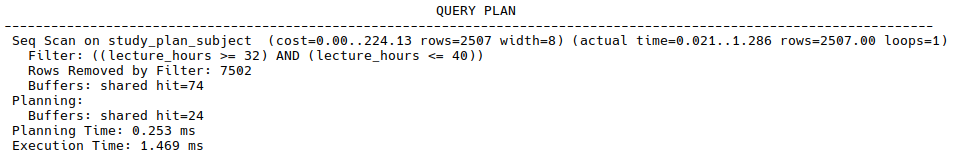
\includegraphics{q10p1.png}
\end{figure}
\item SQL"=код спроектированных индексов:
\begin{minted}{sql}
CREATE INDEX idx_lecture_hours ON study_plan_subject(lecture_hours)
WHERE lecture_hours >= 30;
\end{minted}
\item Скриншот планов выполнения запросов с индексом:
\begin{figure}
\centering
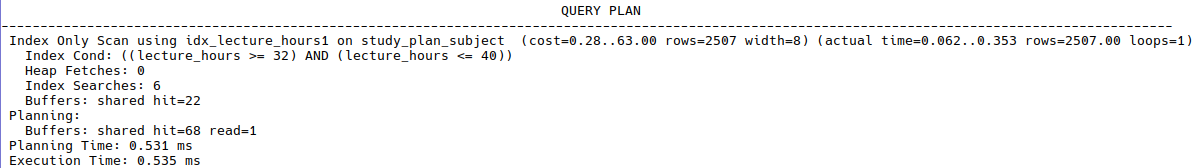
\includegraphics{q10p2.png}
\end{figure}
\end{enumerate}

\subsection{Hash}

\subsubsection{Запрос 1}

\begin{enumerate}
\item Код запроса:
\begin{minted}{sql}
EXPLAIN ANALYZE
SELECT name, surname, passport
FROM students
WHERE group_id = 1 AND name = 'Иван';
\end{minted}
\item Скриншот планов выполнения запросов без индекса:
\begin{figure}
\centering
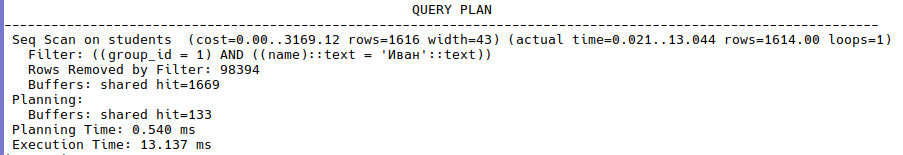
\includegraphics{q16p1.png}
\end{figure}
\item SQL"=код спроектированных индексов:
\begin{minted}{sql}
CREATE INDEX idx_name_partial ON students USING HASH (name)
WHERE group_id = 1;
\end{minted}
\item Скриншот планов выполнения запросов с индексом:
\begin{figure}
\centering
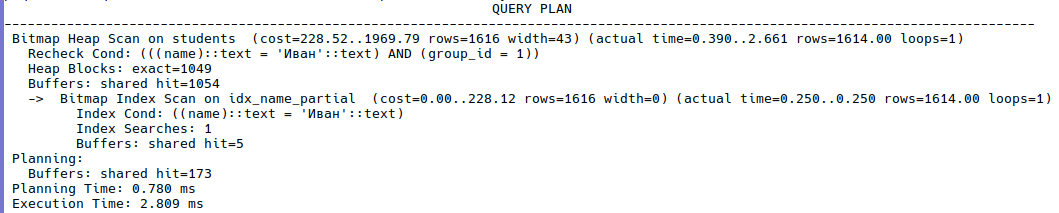
\includegraphics{q16p2.png}
\end{figure}
\end{enumerate}


\section{Частичный покрывающий индекс}
\subsection{B"=Tree}

\subsubsection{Запрос 1}

\begin{enumerate}
\item Код запроса:
\begin{minted}{sql}
EXPLAIN ANALYZE
SELECT student_id, order_type,
       CURRENT_TIME AS access_time,
       CURRENT_TIMESTAMP AS access_timestamp,
       CURRENT_TIMESTAMP::TIMESTAMP WITHOUT TIME ZONE AS access_timestamp_without_tz 
FROM student_orders
WHERE order_date >= LOCALTIMESTAMP - INTERVAL '7 days' AND student_id BETWEEN 100 AND 1000;
\end{minted}
\item Какие типы запросов реализует?
\begin{itemize}
    \item фильтрация данных в запросах с использованием предикатов: BETWEEN;
    \item Запросы с использованием функций даты и времени: арифметические операции с датами, CURRENT\_TIMESTAMP с уточнением временной зоны и без.
\end{itemize}
\item Скриншот планов выполнения запросов без индекса:
\begin{figure}
\centering
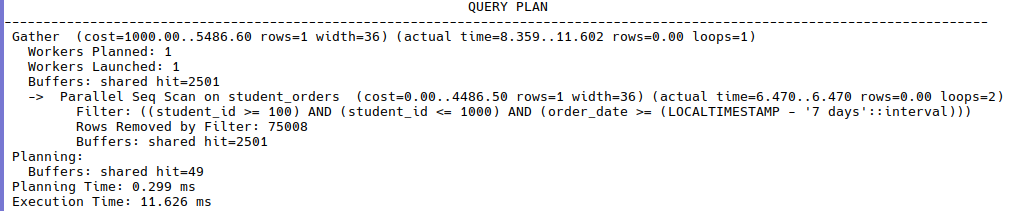
\includegraphics{q14p1.png}
\end{figure}
\item SQL"=код спроектированных индексов:
\begin{minted}{sql}
CREATE INDEX idx_order_date ON student_orders(order_date) INCLUDE (student_id, order_type)
WHERE student_id <= 1000;
\end{minted}
\item Скриншот планов выполнения запросов с индексом:
\begin{figure}
\centering
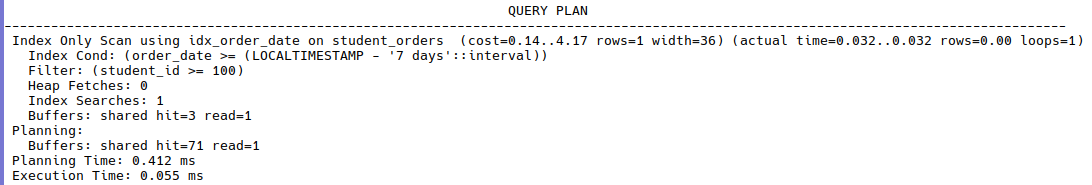
\includegraphics{q14p2.png}
\end{figure}
\end{enumerate}

%После введения — серии \section, \subsection и т.д.

% \conclusion

% Отобразить все источники. Даже те, на которые нет ссылок.
% \nocite{*}

\bibliographystyle{ugost2008}
\bibliography{thesis}

% Окончание основного документа и начало приложений Каждая последующая секция
% документа будет являться приложением
\appendix

\end{document}
